%% The first command in your LaTeX source must be the \documentclass command.
%%
%% Options:
%% twocolumn : Two column layout.
\documentclass[cte]{acnsart}

\setdoi{10.55056/cte.927}
\setjournalyear{2025}
\setjournalvolume{12}
\setcounter{page}{78}


\begin{document}



%%
%% The ``title'' command
\title{Gamification as a tool for developing digital competence in higher education: Theory, practice, and implementation guidelines}

%%
%% The ``author'' command and its associated commands are used to define
%% the authors and their affiliations.
\author[1]{Liubov O. Titova}[%
orcid=0000-0002-2441-0560,
]
\ead{l.o.titova@udpu.edu.ua}
%\ead[url]{http://philosophy.kpi.ua/vikladachi/pokulyta-iryna-kostyantynivna/}

\address[1]{Pavlo Tychyna Uman State Pedagogical University, 2 Sadova Str., Uman, 20300, Ukraine}

\author[2]{Serhii S. Korniienko}[%
orcid={0000-0002-2573-2115},
email={korniienko.serhii@kdpu.edu.ua},
]

\author[2]{Pavlo V. Zahorodko}[%
orcid={0000-0002-8254-7899},
email={zahorodko.pavlo@kdpu.edu.ua},
]


	\author[2]{Mykhailo V. Moiseienko}[%
orcid={0000-0003-4401-0297},
email={seliverst17moiseenko@gmail.com},
url={https://kdpu.edu.ua/personal/mvmoiseienko.html}
]

\address[2]{Kryvyi Rih State Pedagogical University,
	54 Universytetskyi Ave., Kryvyi Rih, 50086, Ukraine}



\author[3]{Ivan I. Donchev}[
orcid={0000-0002-3373-6562}, 
email={donchev@pdpu.edu.ua},
%url={https://kdpu.edu.ua/personal/obkanevska.html}
]

\address[3]{South Ukrainian National Pedagogical University named after K. D. Ushynsky, 26 Staroportofrankivska Str., Odesa,
	65020, Ukraine}


%\author{Olha V. Sotska}[%
%]
%\ead{olyasotskaya03@gmail.com}

%\author[2]{Ivan G. Riznitskii}[%
%]
%\ead[url]{http://nmetau.edu.ua/ua/mdiv/i2051/p-2/e2196}
%\address[2]{State University of Economics and Technology, 5 Stepana Tilhy Str., Kryvyi Rih, 50006, Ukraine}

%%
%% The abstract is a short summary of the work to be presented in the
%% article.
\begin{abstract}
This paper explores the role of gamification as a means of developing digital competence among higher education students. In today's information-driven world, digital competence has become essential for both personal and professional success. The paper analyses the components of digital competence according to the DigComp 2.0 framework and examines how gamification principles can be effectively applied to develop these competencies. A detailed case study of PC Building Simulator implementation in an Informatics course is presented, demonstrating how this gamified approach addresses multiple dimensions of digital competence development. The integration of augmented reality technology further enhances the learning experience. Drawing on contemporary research, the paper offers implementation guidelines, explores cross-disciplinary applications, and outlines a future research agenda for gamification in higher education. The findings suggest that when thoughtfully designed and implemented, gamification approaches can significantly enhance students' motivation and engagement while systematically developing crucial digital competencies required in the modern professional landscape.
\end{abstract}

%%
%% Keywords. The author(s) should pick words that accurately describe
%% the work being presented. Separate the keywords with commas.
\begin{keywords}
	gamification \sep digital competence \sep higher education \sep DigComp 2.0 \sep PC Building Simulator \sep simulation-based learning \sep augmented reality \sep student engagement \sep motivation \sep educational technology \sep informatics education \sep cross-disciplinary applications \sep implementation guidelines \sep problem-solving skills \sep digital literacy
\end{keywords}

%%
%% This command processes the author and affiliation and title
%% information and builds the first part of the formatted document.
\maketitle

\section{Introduction}



\subsection{Research problem and relevance}

In an era where digital technologies permeate virtually every aspect of modern society, the development of digital competence has transitioned from being merely beneficial to absolutely essential. Higher education institutions worldwide face the challenge of preparing graduates who are not only knowledgeable in their specific disciplines but also possess the digital skills needed to thrive in an increasingly technology-dependent professional landscape \cite{Barboutidis2023613}. Despite this recognised importance, many educational programmes struggle to integrate digital competence development in ways that are engaging, comprehensive, and aligned with contemporary learning preferences \cite{Guitert2023245}.

The traditional approaches to developing digital skills often rely heavily on direct instruction, isolated technology courses, or incidental learning through general technology use. Such approaches frequently fail to engage learners deeply or to address the multifaceted nature of digital competence as articulated in frameworks like DigComp 2.0 \cite{Vuorikari2016}. Consequently, there is growing interest in innovative pedagogical approaches that can more effectively foster the development of these crucial competencies.

Gamification~-- the application of game elements and design principles in non-game contexts~-- has emerged as a promising approach to address these challenges \cite{Deterding2011}. By harnessing the motivational power of games whilst maintaining focus on educational objectives, gamification offers a framework for creating engaging learning experiences that align with the preferences of today's digitally-oriented students. Recent studies indicate that gamification can significantly enhance student engagement, motivation, and learning outcomes when thoughtfully integrated into educational contexts \cite{Humeniuk2022113, Mitchell2024184}.

The intersection of gamification and digital competence development represents a particularly promising area of educational innovation, yet comprehensive research exploring this intersection remains relatively scarce. This gap in the literature presents an opportunity to advance understanding of how gamification approaches can be systematically applied to foster specific dimensions of digital competence in higher education settings.

\subsection{Aims and objectives}

This paper aims to explore and articulate the potential of gamification as a pedagogical approach for developing digital competence in higher education students. The specific objectives of the study are to:

\begin{enumerate}[1)]
\item analyse the components of digital competence as defined by contemporary frameworks, with particular reference to DigComp 2.0;
\item examine the theoretical foundations and key elements of gamification as an educational approach;
\item establish conceptual connections between gamification principles and digital competence development;
\item present and analyse a detailed case study of PC Building Simulator implementation in an Informatics course, illustrating how this gamified approach addresses multiple dimensions of digital competence;
\item develop practical guidelines for implementing gamification approaches to foster digital competence in higher education settings;
\item explore potential cross-disciplinary applications of simulation-based gamification approaches; %and
\item identify key research gaps and future directions for this field of educational innovation.
\end{enumerate}

\subsection{Methodology and scope}

This research employs a mixed methodological approach combining theoretical analysis, case study examination, and synthesis of contemporary research literature. The theoretical analysis involves a detailed examination of digital competence frameworks and gamification principles to establish conceptual connections between these domains. The case study component focuses on the implementation of PC Building Simulator in an Informatics course at Pavlo Tychyna Uman State Pedagogical University, providing concrete illustration of the application of gamification principles for digital competence development.

The paper draws on a review of scholarly literature on gamification in higher education, digital competence development, and educational simulation technologies published predominantly within the past decade. This literature base encompasses empirical studies, theoretical analyses, systematic reviews, and implementation reports published in peer-reviewed journals and conference proceedings.

The scope of this paper is limited to higher education contexts, with particular emphasis on undergraduate level education. While the primary case study involves students in mathematics and computer science education programmes, the paper also explores potential applications in other disciplinary contexts. The focus is primarily on simulation-based gamification approaches, though other gamification strategies are considered where relevant to digital competence development.

\section{Theoretical foundations}

\subsection{Digital competence in the modern educational context}

%\subsubsection{Evolution of digital competence frameworks}

The concept of digital competence has evolved significantly over recent decades, reflecting the rapidly changing technological landscape and growing recognition of the multifaceted nature of digital skills. Early frameworks often emphasised basic computer operation and software usage~-- what might be termed `computer literacy' or `ICT skills' \cite{Siiman2017148}. However, as digital technologies have become more pervasive and complex, understanding of digital competence has expanded to encompass a much broader range of knowledge, skills, and attitudes.

Contemporary conceptualisations of digital competence recognise that effective engagement with digital technologies requires not only technical proficiency but also critical understanding, ethical awareness, and creative application. This evolution is evident in the development of comprehensive frameworks such as DigComp in Europe, the ISTE Standards internationally, and various national digital competence frameworks worldwide. These frameworks increasingly recognise digital competence as a transversal key competence that intersects with and supports development in virtually all other domains of learning and professional practice \cite{Barboutidis2023613}.

The evolution of these frameworks has been shaped by both theoretical advances in understanding digital literacy and practical observations of how digital technologies are transforming professional practice across disciplines. This dynamic interplay between theory and practice continues to refine our understanding of what constitutes digital competence in the 21st century.

%\subsubsection{DigComp 2.0 Framework Components and Structure}

The European Digital Competence Framework for Citizens, known as DigComp, represents one of the most comprehensive and widely adopted frameworks for conceptualising digital competence. The framework's 2.0 version, released in 2016, identifies five key competence areas, each encompassing several specific competencies \cite{Vuorikari2016}.

The first area, Information and Data Literacy, involves the ability to articulate information needs, locate and retrieve digital data and information, judge its relevance and reliability, and organise and process digital data. This fundamental area forms the foundation for effective engagement with digital information ecosystems.

Communication and Collaboration, the second area, encompasses interaction through digital technologies, sharing of digital content, civic participation via digital channels, collaboration through digital technologies, netiquette, and management of digital identity. These competencies reflect the increasingly social and collaborative nature of digital engagement.

The third area, Digital Content Creation, includes developing and editing digital content, integrating and re-elaborating existing content, understanding copyright and licensing, and programming. These competencies enable productive and creative engagement with digital technologies rather than merely passive consumption.

Safety, the fourth area, covers protection of devices, personal data, privacy, health and well-being, and the environment. This dimension acknowledges the potential risks associated with digital engagement and the importance of protective measures.

Finally, Problem Solving involves resolving technical problems, identifying needs and technological responses, creatively using digital technologies, identifying digital competence gaps, and computational thinking. These competencies enable adaptive and innovative responses to novel digital challenges.

The DigComp 2.0 framework conceptualises each competence area at eight proficiency levels, ranging from foundation to highly specialised, providing a nuanced developmental pathway for each competence. This sophisticated structure makes the framework particularly valuable for educational planning and assessment.

%\subsubsection{Digital Competence in Higher Education}

The importance of digital competence in higher education contexts has grown exponentially in recent years, accelerated further by the global shift toward online and hybrid learning during the COVID-19 pandemic \cite{Vanessa2024444}. Higher education institutions increasingly recognise that digital competence is essential not only for academic success but also for preparing students for professional environments characterised by rapid technological change.

Digital competence in higher education operates at multiple levels. At the most basic level, students require digital competence to effectively engage with institutional learning systems, access digital resources, and complete digitally-mediated assignments. At a more advanced level, discipline-specific digital competencies are often required, such as specialised software applications, data analysis tools, or digital design platforms relevant to particular fields of study.

Beyond these instrumental dimensions, higher education increasingly emphasises critical digital competence~-- the ability to evaluate digital sources, understand the ethical implications of digital practices, and engage thoughtfully with issues of digital privacy, security, and identity. This critical dimension becomes particularly important in preparing students to be informed digital citizens and ethical professionals \cite{Guitert2023245}.

The development of digital competence in higher education presents both opportunities and challenges. On one hand, today's students often enter higher education with significant experience of digital technologies from their personal lives. On the other hand, research consistently shows that this experience does not always translate into the types of digital competencies required for academic and professional success \cite{Barboutidis2023613}. This gap highlights the importance of systematic approaches to developing digital competence within higher education curricula.

\subsection{Gamification in education}

%\subsubsection{Defining Gamification: Key Concepts and Elements}

Gamification refers to the application of game design elements and principles in non-game contexts \cite{Deterding2011}. In educational settings, gamification involves incorporating elements such as points, badges, leaderboards, challenges, narratives, and feedback systems into learning activities without transforming them into full-fledged games. The fundamental premise of gamification is that the motivational power of well-designed games can be harnessed to enhance engagement and motivation in educational contexts.

The components of gamification can be broadly categorised into dynamics, mechanics, and aesthetics, following the MDA (Mechanics, Dynamics, Aesthetics) framework commonly used in game design \cite{Bozic2024538}. Mechanics include the basic rules, actions, and control mechanisms that define how players interact with the system~-- elements such as points, levels, challenges, and rewards. Dynamics represent the run-time behaviour of mechanics as they respond to player inputs~-- the emergent patterns of interaction that develop during use. Aesthetics encompass the emotional responses evoked in users through their interaction with the system~-- feelings of achievement, competition, collaboration, or discovery.

In educational gamification, these elements are carefully selected and integrated to support specific learning objectives while enhancing motivation and engagement. The selection of particular gamification elements should be guided by pedagogical considerations rather than merely transplanting features from popular games \cite{Prieto-Andreu2024244}.

%\subsubsection{Distinguishing Gamification from Other Game-Based Approaches}

While gamification shares common ground with other game-based approaches to education, it is important to distinguish it from related but distinct approaches such as serious games, game-based learning, and simulation games. Serious games are complete games designed for purposes beyond entertainment, often with specific educational objectives. Game-based learning uses full games (either commercial or educational) as primary teaching tools. Simulation games replicate real-world systems or processes in game formats to facilitate understanding through interactive experience.

Gamification, in contrast, does not involve creating or using complete games but rather applying selected game elements to existing educational activities or environments. The core activities remain educational rather than game-based, but they are enhanced with game elements to increase engagement and motivation \cite{Humeniuk2022113}. This distinction is crucial for understanding both the affordances and limitations of gamification as an educational approach.

A key difference lies in the relationship between gameplay and learning objectives. In serious games and game-based learning, the gameplay itself is typically designed to directly teach content or develop skills. In gamification, the game elements are often layered onto existing learning activities, creating a motivational framework around them rather than replacing them \cite{Mitchell2024184}. This makes gamification potentially easier to implement within existing educational structures but may limit its transformative potential compared to more comprehensive game-based approaches.

%\subsubsection{Theoretical Models Supporting Gamification in Learning}

Several theoretical perspectives inform the application of gamification in educational contexts. Self-Determination Theory (SDT) provides a particularly useful framework for understanding how gamification can enhance motivation \cite{Gupta2022341}. SDT identifies three innate psychological needs that drive intrinsic motivation: autonomy (the need to feel control over one's actions), competence (the need to feel effective and capable), and relatedness (the need to feel connected to others). Well-designed gamification can address these needs by providing choices (autonomy), clear progression and achievement systems (competence), and social or collaborative elements (relatedness).

Flow Theory, developed by Csikszentmihalyi, offers another valuable perspective \cite{Ho2024139}. This theory describes an optimal state of immersive engagement where challenge and skill are balanced, goals are clear, feedback is immediate, and self-consciousness disappears. Gamification can be designed to foster flow states by providing appropriate levels of challenge, clear objectives, and immediate feedback~-- all characteristic elements of effective games.

Behaviourist perspectives also inform aspects of gamification, particularly the use of rewards and feedback systems \cite{Nunez-Naranjo2024106}. While an exclusively behaviourist approach risks undermining intrinsic motivation, carefully designed reward systems can support learning when they provide informational feedback rather than mere external control.

More recently, the Octalysis framework has emerged as a comprehensive model specifically for gamification design \cite{Ho2024139}. This framework identifies eight core drives of motivation: epic meaning and calling, development and accomplishment, empowerment of creativity and feedback, ownership and possession, social influence and relatedness, scarcity and impatience, unpredictability and curiosity, and loss and avoidance. The framework provides a structured approach to designing gamification that addresses multiple motivational factors.

%\subsubsection{Motivation and Engagement Through Gamification}

A primary rationale for implementing gamification in education is its potential to enhance student motivation and engagement. Research consistently indicates that well-designed gamification can increase participation, time on task, and persistence in learning activities \cite{Mitchell2024184, Zainuddin20241261}. These effects appear particularly pronounced for students who initially demonstrate lower levels of motivation or engagement with traditional instructional approaches.

The motivational impact of gamification operates through several mechanisms. Immediate feedback systems provide continual reinforcement of progress, helping students maintain momentum and adjust their approaches as needed. Achievement systems such as points, badges, and levels make progress visible and satisfying, converting abstract learning gains into concrete markers of achievement. Challenge structures provide optimal difficulty levels that maintain engagement without overwhelming learners. Narrative elements can contextualise learning within meaningful stories that increase emotional investment. Social elements like teams, competition, or collaboration leverage social motivations to enhance individual engagement \cite{Humeniuk2022113}.

However, research also indicates important nuances in the motivational effects of gamification. Different gamification elements may affect different types of motivation, with potential tensions between intrinsic and extrinsic motivational factors \cite{Ho2024139}. For example, extrinsic rewards may undermine intrinsic motivation in some contexts while enhancing it in others, depending on how they are implemented and perceived. Furthermore, individual differences in personality, learning preferences, and prior gaming experience can significantly moderate the effects of gamification on motivation and engagement \cite{Prieto-Andreu2024244}.

These complexities highlight the importance of thoughtful design in educational gamification. Rather than applying game elements indiscriminately, effective gamification requires careful consideration of learning objectives, student characteristics, and motivational dynamics. When designed with these considerations in mind, gamification offers significant potential for enhancing the motivational dimensions of higher education learning experiences.

\section{Mapping gamification elements to digital competence development\label{sec3}}

The integration of gamification principles with digital competence development represents a promising educational approach, yet requires thoughtful alignment between specific gamification elements and the competence areas they aim to develop. This section examines how various gamification strategies and elements can be mapped to the five key areas of digital competence identified in the DigComp 2.0 framework.

\subsection{Information and data literacy competence through gamification}

Information and data literacy encompasses the abilities to articulate information needs, locate and retrieve digital information, judge its relevance and reliability, and store, manage, and organise digital content. Gamification offers several powerful approaches to developing these competencies in higher education contexts.

Quest-based gamification structures can effectively develop information search and evaluation skills by presenting students with information challenges that require them to locate, evaluate, and synthesise digital information from various sources. For example, digital scavenger hunts can require students to locate specific types of information using different search strategies, with points awarded for both efficiency and the quality of sources identified. Progressive difficulty levels can gradually introduce more complex information needs and more specialised information sources, mirroring the developmental progression outlined in the DigComp framework.

Badges and achievement systems can be effectively aligned with specific information literacy skills, such as ``Advanced Searcher'' badges for demonstrating proficiency with advanced search operators, or ``Critical Evaluator'' achievements for successfully identifying misleading information or biased sources. These visible markers of achievement not only motivate skill development but also make abstract information literacy competencies more concrete and measurable.

Simulation environments can provide safe spaces for practising information management skills, allowing students to experiment with different approaches to organising and retrieving digital information. For instance, simulated research projects can require students to develop information management systems that they must later use to retrieve specific information under time constraints, making the practical value of effective information organisation immediately apparent.

Research by \citet{Flores-Bueno2021} demonstrates that gamification can significantly improve information literacy skills among university students, with particularly strong effects on source evaluation and information organisation abilities. Their study found that gamified approaches led to greater skill transfer to authentic information tasks compared to traditional information literacy instruction.

\subsection{Communication and collaboration through gamified learning}

The communication and collaboration area of digital competence involves interacting through digital technologies, sharing digital content, engaging in online citizenship, collaborating through digital channels, managing digital identity, and practising appropriate online behaviour (netiquette). Gamification offers numerous opportunities to develop these competencies through structured social interactions and collaborative challenges.

Team-based gamification structures naturally support the development of digital collaboration skills by requiring students to coordinate their efforts through digital tools. For example, team challenges can require coordinated problem-solving through digital communication channels, with points or advancement contingent on effective information sharing and task coordination. Such approaches develop not only technical proficiency with collaboration tools but also the social and procedural knowledge required for effective digital collaboration.

Role-playing elements can be particularly effective for developing competencies related to digital identity and netiquette. By assuming different digital roles or personas within gamified environments, students can experience different perspectives on digital interaction and develop awareness of how identity is constructed and perceived online. For instance, students might take turns assuming the roles of different stakeholders in online discussions, earning points for appropriate communication that considers the specific context and audience.

Leaderboards and social recognition systems can be designed to reward positive contributions to digital communities rather than merely individual achievement. For example, peer rating systems can award points for helpful contributions to class forums, respectful engagement in online debates, or effective knowledge sharing. These systems make the often invisible social dimensions of digital competence visible and valued.

Research by \citet{Barboutidis2023613} found that age and specialisation significantly affect the communication and collaboration area of digital competence, with younger students and those in certain technical fields demonstrating higher baseline competence. However, their research also indicated that gamification could effectively reduce these gaps by providing structured opportunities for all students to develop and practise communication and collaboration skills in digital contexts.

\subsection{Digital content creation skills via gamification}

Digital content creation competencies include creating and editing digital content, integrating and re-elaborating existing content, understanding copyright and licenses, and programming. Gamification approaches can scaffold the development of these creative and technical skills while making the learning process more engaging and less intimidating.

Challenge-based gamification structures provide excellent frameworks for developing digital creation skills by breaking complex creation processes into manageable stages with clear objectives and feedback. For example, digital media creation challenges can progress from simple editing tasks to more complex multimedia productions, with each level introducing new tools and techniques. This staged approach helps overcome the initial reluctance or anxiety many students feel when faced with unfamiliar creative tools or programming environments.

Achievement systems can effectively track mastery of specific creation tools and techniques, providing visible recognition of skill development. For instance, badges can be awarded for demonstrating proficiency with specific software features, successfully implementing particular programming concepts, or creating specific types of digital content. This approach helps students build confidence through a series of small, recognised accomplishments.

Competitive and collaborative creation challenges can motivate higher levels of engagement with content creation tools. For example, time-limited creation challenges can inspire creative applications of digital tools, while collaborative creation projects can leverage social motivation to encourage exploration of more advanced features and techniques. These approaches help students move beyond basic tool operations to develop more sophisticated creation skills.

Particularly relevant to higher education contexts is the use of gamification to develop understanding of copyright, licensing, and intellectual property issues in digital contexts. Interactive scenarios can present students with realistic copyright dilemmas, awarding points for correctly identifying and navigating complex intellectual property issues. This approach develops not only knowledge of relevant laws and policies but also the judgement required to apply this knowledge in ambiguous real-world situations.

According to \citet{Barboutidis2023613}, educational level significantly affects digital content creation competencies, making this an area where gamification may be particularly beneficial in higher education contexts. Their research suggests that gamified approaches can help students transition from basic content manipulation to more sophisticated creation and integration skills.

\subsection{Safety competencies and gamification}

The safety dimension of digital competence encompasses protecting devices and digital content, safeguarding personal data and privacy, protecting health and well-being, and addressing environmental impacts of digital technologies. Gamification offers unique opportunities to develop these competencies through simulated experiences and decision-making scenarios.

Simulation-based gamification provides particularly powerful approaches for developing device and data security competencies. For example, cybersecurity simulations can place students in realistic scenarios where they must identify and respond to potential security threats, with points or advancement contingent on correct identification and appropriate responses. These simulated experiences allow students to develop security awareness and practise protective behaviours without actual risk.

Scenario-based challenges can effectively develop privacy management competencies by presenting students with realistic privacy dilemmas that require them to evaluate privacy implications and make appropriate decisions. For instance, students might navigate scenarios involving social media sharing, app permissions, or data collection practices, earning points for decisions that appropriately balance functionality with privacy protection. This approach helps students develop nuanced judgement rather than simply memorising privacy rules.

Health and well-being aspects of digital safety can be addressed through gamified tracking and reflection activities. For example, students might earn points or achievements for maintaining healthy technology use patterns or implementing ergonomic best practices. These approaches help develop self-regulation skills and awareness of the physical and psychological impacts of digital technology use.

Environmental aspects of digital safety can be addressed through simulation games that visualise the environmental impacts of digital choices and reward sustainable digital practices. For example, simulations might demonstrate the energy consumption and carbon impacts of different data storage or processing approaches, with rewards for identifying and implementing more sustainable alternatives.

Research by \citet{Vuorikari2016} emphasises that safety competencies extend beyond technical knowledge to encompass attitudinal and behavioural dimensions, making them particularly well-suited to gamification approaches that can engage students emotionally and provide practice in applied decision-making. Gamification can help bridge the common gap between knowledge of safety best practices and their consistent application.

\subsection{Problem-Solving competence development through gamified approaches}

Problem-solving in the context of digital competence involves resolving technical issues, identifying needs and finding technological solutions, using digital technologies creatively, identifying digital competence gaps, and computational thinking. These complex competencies benefit particularly from gamification approaches that provide structured yet open-ended problem spaces.

Challenge-based gamification structures naturally align with problem-solving competence development by presenting students with increasingly complex technical challenges that require analytical thinking and creative solutions. For example, troubleshooting challenges can present students with realistic technical problems that they must diagnose and resolve, with points or advancement reflecting the efficiency and effectiveness of their solutions. This approach develops not only technical knowledge but also the systematic thinking processes essential for effective problem-solving.

Sandbox environments with gamified elements provide excellent contexts for developing creative technology use competencies. These environments allow open-ended exploration of digital tools with achievement systems that recognise innovative applications or particularly elegant solutions. This combination of freedom and recognition encourages students to move beyond prescribed uses of digital technologies to develop more flexible and creative approaches.

Progression systems can effectively support the development of computational thinking by guiding students through increasingly complex computational challenges. For example, programming challenges can progress from simple algorithms to more complex problem decomposition and pattern recognition tasks, with each level building on previous concepts while introducing new complexity. This structured progression helps make abstract computational concepts more accessible and engaging.

Particularly relevant to higher education contexts is the use of gamification to develop meta-cognitive awareness of one's own digital competence gaps. Reflection activities with gamified elements can encourage students to accurately assess their own competencies and identify areas for development. For instance, self-assessment activities might award points for honest reflection and realistic goal-setting, encouraging students to take ownership of their ongoing digital competence development.

According to \citet{Barboutidis2023613}, possession and use of PCs significantly affects problem-solving competencies, suggesting that gamification approaches that increase engagement with digital technologies may be particularly beneficial for developing this competence area. Their research indicates that regular, motivated engagement with varied digital challenges is key to developing robust problem-solving competencies.

The mapping of gamification elements to specific digital competence areas provides a framework for designing targeted educational interventions. However, it is important to note that many gamification approaches can address multiple competence areas simultaneously, reflecting the interconnected nature of digital competencies in authentic contexts. Effective implementation requires thoughtful design that considers not only the alignment between game elements and competence areas but also the specific educational context and student characteristics.

\section{Case Study: PC Building Simulator as a tool for digital competence development}

\subsection{Overview of the PC Building Simulator}

PC Building Simulator represents an innovative educational tool that combines simulation technology with gamification principles to create an engaging learning environment for developing various aspects of digital competence. As described by \citet{Alhumairi202422}, simulation-based learning environments offer unique opportunities for experiential learning in technical domains, providing safe spaces for students to develop practical skills through authentic activities.

PC Building Simulator is a game-based simulation environment that allows users to engage with realistic virtual representations of computer hardware components and assembly processes. The simulator includes a comprehensive library of accurately modelled computer components, realistic physics for component interactions, and authentic system behaviour that responds to user actions and configuration choices. These features create a high-fidelity simulation environment that closely mirrors real-world computer assembly and troubleshooting experiences \cite{Alexov2023}.

\begin{figure}[ht]
\centering
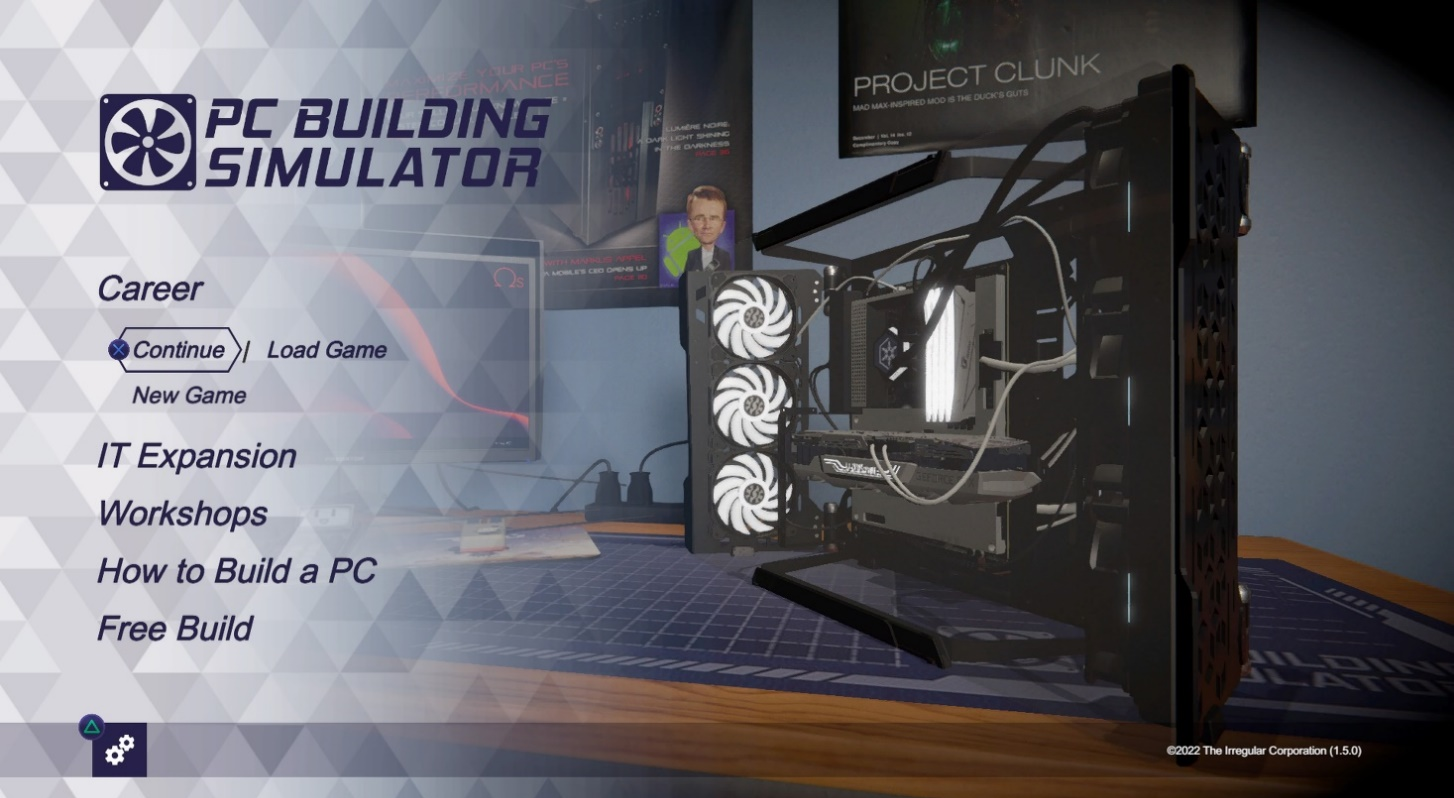
\includegraphics[width=\textwidth]{image1}
\caption{Main window of PC Building Simulator.}
\label{fig:pcbs_main}
\end{figure}

The simulator offers two primary modes of operation, each supporting different learning objectives and engagement patterns. The free-build mode provides unrestricted access to all available components, allowing users to experiment freely with different hardware configurations and assembly processes. This mode supports exploratory learning and creative experimentation without external constraints or objectives. The career mode, in contrast, presents a progression-based experience where users operate a virtual computer repair business, completing increasingly complex client tasks to earn reputation points and in-game currency that unlocks additional components and capabilities. This structured progression implements classic gamification principles, creating a motivational framework around the core simulation activities \cite{Alexov2023}.

As observed by \citet{Wang2016319}, educational simulations are particularly valuable when they combine high-fidelity modelling of technical systems with engaging interaction paradigms that motivate sustained engagement. PC Building Simulator exemplifies this approach, offering both technical accuracy and motivational game elements that encourage extended interaction and deeper learning.

\subsection{Implementation in the Informatics course}

The implementation of PC Building Simulator in the Informatics course for first-year bachelor's students in the ``Secondary Education (Mathematics, Informatics)'' programme at Pavlo Tychyna Uman State Pedagogical University represents a thoughtful integration of gamification principles into an existing curriculum structure. This implementation specifically targeted the ``Hardware and Software of Information Systems'' module, using the simulator to transform traditionally abstract and theoretical content into an interactive, experiential learning opportunity.

The implementation followed a structured approach to ensure alignment with existing course objectives while leveraging the unique affordances of the simulation environment. Prior to introducing the simulator, students received foundational instruction on basic computer architecture concepts and component functions, establishing a theoretical framework that would later be applied and expanded through the simulation activities. This approach aligns with \citet{Zweifel20171103}'s recommendation that simulation technologies be introduced after establishing basic conceptual understanding to maximise their educational value.

The instructional design incorporated both individual and collaborative elements. Students initially engaged with the simulator individually, completing guided exploration activities that familiarised them with the interface and basic functionality. These activities gradually increased in complexity, from simple component identification to complete system assembly and configuration. Following this individual orientation, collaborative challenges were introduced, requiring student teams to design systems meeting specific performance requirements or troubleshoot deliberately problematic configurations. This combination of individual and collaborative activities supports the development of both technical competencies and the collaborative skills identified in the DigComp framework \cite{Vuorikari2016}.

Assessment was integrated throughout the implementation, combining traditional knowledge assessment with performance-based evaluation within the simulation environment. Students were evaluated not only on their theoretical understanding of computer hardware concepts but also on their practical ability to apply this knowledge in the simulator. Assessment tasks included efficient system assembly, accurate troubleshooting, optimal component selection for specific use cases, and explanation of configuration decisions. This multifaceted assessment approach aligns with \citet{Adams2022119}'s recommendation that gamified learning environments include assessment strategies that capture both knowledge and applied competencies.

The implementation was supported by customised instructional materials that bridged the simulator activities and course learning objectives. These materials included guided worksheets that directed student attention to key concepts during simulation activities, reflection prompts that encouraged metacognitive processing of simulation experiences, and supplementary resources that connected simulation activities to broader theoretical frameworks. As noted by \citet{Figg20181215}, such supporting materials are crucial for ensuring that gamification elements enhance rather than distract from core learning objectives.

\subsection{Enhancing learning with augmented reality}

A particularly innovative aspect of the PC Building Simulator implementation was the integration of augmented reality (AR) technology through the use of AR headsets connected to PlayStation 4 Pro systems, creating an immersive learning environment that further enhanced student engagement and learning outcomes. This technological integration represents a cutting-edge approach to educational gamification, combining simulation, gaming, and immersive technologies to create a uniquely powerful learning experience.

\begin{figure}[ht]
\centering
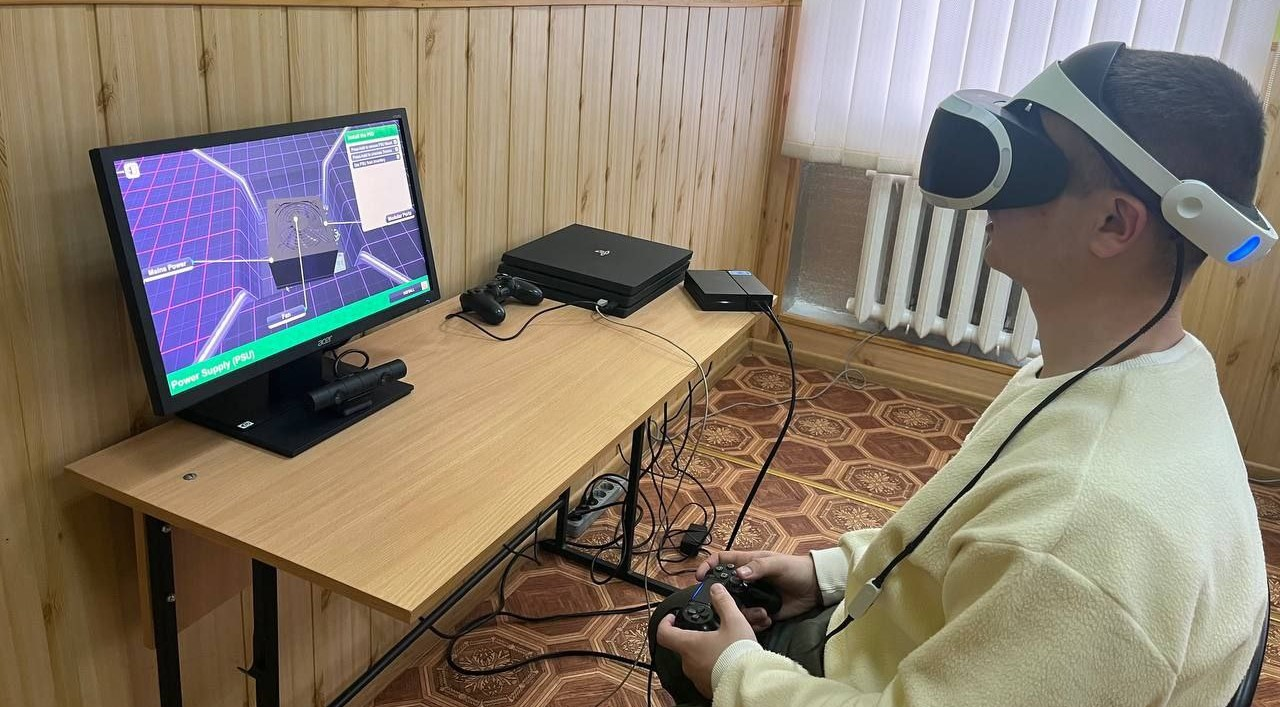
\includegraphics[width=\textwidth]{image3}
\caption{Learning PC structure using AR technology.}
\label{fig:ar_learning}
\end{figure}

The AR implementation allowed students to experience computer hardware components and assembly processes in a three-dimensional virtual space, creating a sense of presence and embodiment that significantly enhanced the experiential dimension of learning. As students navigated the virtual environment, physical movements and hand gestures were translated into virtual interactions with computer components, creating a more intuitive and engaging interface compared to traditional mouse and keyboard controls. This approach aligns with  findings by \citet{Li2024} that immersive virtual environments can significantly enhance spatial understanding and procedural knowledge acquisition in technical domains.

The AR integration addressed several key educational challenges identified in previous research on computer hardware education. Traditional approaches to teaching computer hardware concepts often struggle to provide students with hands-on experience due to the cost of components, risk of damage to physical hardware, and limited opportunity for experimentation with diverse configurations. AR technologies allow students to ``fully immerse themselves in the process and learn the structure of the PC more thoroughly'' without these constraints, creating a safe environment for exploration and experimentation that would be impractical or impossible with physical hardware.

From a pedagogical perspective, the AR integration leveraged the principle of embodied cognition, which suggests that physical interaction with learning materials can enhance conceptual understanding and retention. Students reported that the ability to ``reach out and grab'' virtual components created a more intuitive understanding of spatial relationships and assembly procedures compared to traditional screen-based interactions. This aligns with observation of \citet{Alhumairi202422} that immersive technologies can create deeper encoding of procedural knowledge through physical engagement with learning activities.

The implementation was not without challenges, however. Some students experienced initial disorientation or motion sickness during AR sessions, requiring careful orientation and progressive introduction to the immersive environment. Additionally, the AR hardware introduced logistical complexities for class management, requiring dedicated training for instructional staff and careful scheduling to ensure equitable access for all students. These implementation challenges echo those identified by \citet{Alhumairi202422} in their study of VR implementation in computer science education, suggesting common barriers that must be addressed when integrating immersive technologies in educational settings.

Despite these challenges, the AR integration significantly enhanced the educational value of the PC Building Simulator implementation, creating a more engaging and effective learning environment for developing digital competencies. As noted by \citet{Kalua2020}, ``the integration of simulation and immersive technologies creates synergistic effects that exceed the educational value of either approach in isolation'', a principle clearly demonstrated in this implementation.

\subsection{Addressing digital competence areas through the simulator}

\subsubsection{Hardware knowledge and information literacy}

PC Building Simulator provides a structured environment for developing information literacy competencies related to computer hardware knowledge. Students must locate, evaluate, and apply information about hardware components and their compatibility, developing critical information processing skills in an authentic context. As students interact with the simulator's virtual component library, they learn to interpret technical specifications, compare alternative components, and make informed decisions based on performance requirements and compatibility constraints.

The simulator's component database provides a realistic information environment that mirrors the complexity of real-world hardware information ecosystems. Students must navigate this information landscape, learning to distinguish between critical and secondary specifications, recognise compatibility issues, and evaluate the reliability of performance claims. These activities directly address the information and data literacy competence area identified in the DigComp framework, particularly the abilities to ``search for data, information and content in digital environments'' and to ``analyse, compare and critically evaluate the credibility and reliability of data sources'' \cite{Vuorikari2016}.

Furthermore, the simulator's career mode presents information challenges of progressively increasing complexity, mirroring the developmental progression outlined in the DigComp framework. Initial tasks require only basic information processing, while advanced challenges demand sophisticated comparison and evaluation of multiple information sources to devise optimal solutions. This structured progression helps students develop increasingly advanced information literacy skills through guided practice in authentic contexts.

\subsubsection{Technical problem-solving}

The problem-solving dimension of digital competence is particularly well-addressed through PC Building Simulator's troubleshooting activities. In the career mode, students encounter a variety of technical problems ranging from basic hardware incompatibilities to complex system performance issues. Resolving these problems requires systematic diagnostic approaches, analytical thinking, and creative application of technical knowledge~-- all core components of digital problem-solving competence.

\begin{figure}[ht]
\centering
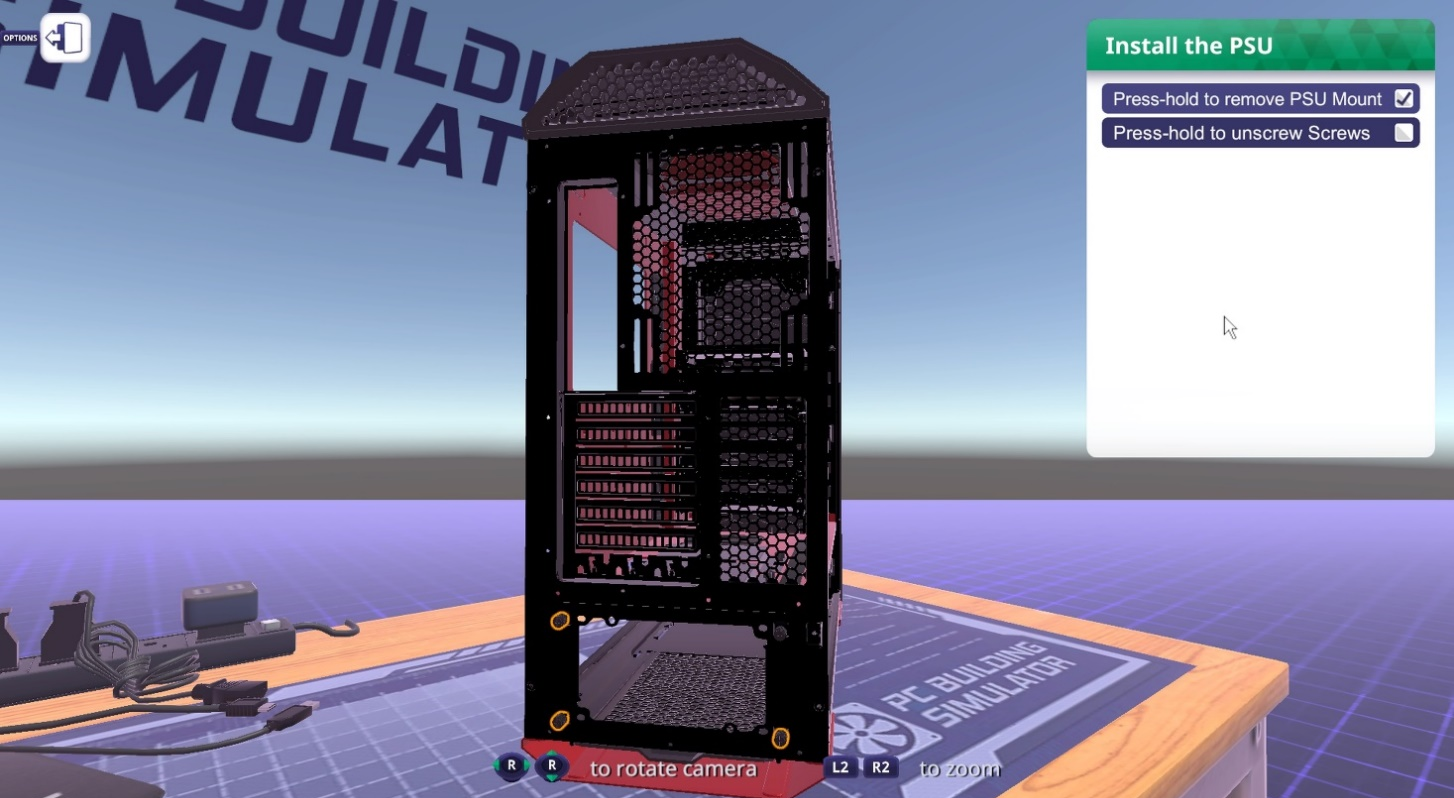
\includegraphics[width=\textwidth]{image2}
\caption{Step-by-step instruction for PC assembly.}
\label{fig:assembly_instruction}
\end{figure}

The simulator provides a safe environment for developing these problem-solving skills, allowing students to experience the consequences of their diagnostic decisions without risk to physical hardware. This ``safe failure'' environment encourages experimental approaches and helps students develop resilience and confidence when facing technical challenges. As \citet{Kivits2013} notes, such simulation environments ``allow learners to develop robust problem-solving strategies through repeated practice and immediate feedback on the consequences of their actions''.

Particularly valuable is the simulator's representation of complex system interdependencies that mirror real-world troubleshooting challenges. Students learn that technical problems often have multiple potential causes and that diagnostic processes must consider the system holistically rather than focusing only on isolated components. This systems thinking approach represents a sophisticated form of digital problem-solving that transfers readily to other technical domains.

\subsubsection{Digital content management}

While less immediately obvious, PC Building Simulator also addresses aspects of the digital content creation competence area, particularly related to digital content management and system configuration. Within the simulator, students create and manage virtual operating system environments, installing and configuring software, managing virtual file systems, and optimising system configurations for specific use cases.

These activities develop practical understanding of digital content management principles and processes. Students learn how digital content interacts with hardware systems, how system configurations affect content performance, and how to optimise environments for different types of digital content creation and consumption. This practical understanding complements more abstract instruction on digital content creation, grounding theoretical concepts in concrete examples of system-content interactions.

The simulator also introduces students to basic concepts of digital rights management and software licensing through its representation of operating system and application installation processes. Students encounter realistic software licensing scenarios and learn to navigate the legal and technical aspects of software installation and management~-- an increasingly important aspect of digital content competence in professional contexts.

\subsubsection{Digital safety awareness}

The safety dimension of digital competence is addressed through PC Building Simulator's representation of hardware safety considerations and system security concepts. Students learn about proper component handling procedures, power management safety, and protection against electrostatic discharge~-- all essential knowledge for safe interaction with physical computing hardware.

Beyond physical safety, the simulator introduces fundamental concepts of digital security through virtual operating system and antivirus installation activities. Students learn about system vulnerabilities, malware protection, and basic security configuration~-- essential components of the safety competence area identified in the DigComp framework. While not the primary focus of the simulator, these elements help students develop awareness of digital safety issues in the context of system management.

As \citet{Petr2007629} observes, simulation environments can effectively develop safety awareness by allowing students to ``observe the consequences of unsafe practices in a risk-free environment''. This principle is evident in PC Building Simulator, where students can experience the virtual consequences of safety violations without risk to physical hardware or data.

\subsubsection{Communication and collaboration components}

The implementation of PC Building Simulator included collaborative activities that specifically targeted the communication and collaboration area of digital competence. Student teams worked together on complex building challenges, requiring coordinated planning, clear communication of technical information, and collaborative problem-solving~-- all mediated through digital channels.

These collaborative activities developed several specific competencies identified in the DigComp framework, including ``interacting through digital technologies'', ``sharing through digital technologies'', and ``collaborating through digital technologies'' \cite{Vuorikari2016}. Students learned to communicate technical information clearly, coordinate complex technical activities, and leverage digital tools to support collaborative problem-solving.

Particularly valuable was the development of field-specific communication skills related to computer hardware terminology and concepts. Students developed the ability to describe technical issues precisely, document configuration decisions clearly, and explain technical rationales effectively~-- all essential communication skills in technical professional contexts. As \citet{Christiansson200593} notes, such domain-specific communication competencies are crucial for effective professional practice but are often underdeveloped in traditional educational approaches.

\section{Implementation guidelines for gamification in higher education\label{sec5}}

The effective implementation of gamification approaches for developing digital competence requires thoughtful planning, design, and execution. Drawing on both the case study presented in this paper and broader research on educational gamification, this section presents a structured framework for implementing gamification initiatives in higher education settings.

\subsection{Pedagogical framework for gamification integration}

Successful gamification implementation begins with a clear pedagogical framework that aligns game elements with educational objectives and theoretical principles. As emphasised by \citet{Moutinho202122}, ``gamification should be conceived as a pedagogical approach rather than merely a technological intervention'', requiring thoughtful integration with broader educational theories and practices.

A comprehensive pedagogical framework for gamification should address several key dimensions. First, learning objectives must be clearly articulated and prioritised, ensuring that gamification elements serve educational purposes rather than becoming ends in themselves. These objectives should be specific, measurable, and aligned with recognised competency frameworks such as DigComp 2.0 to ensure comprehensive coverage of essential skills.

Second, the framework should incorporate motivational theories that inform the selection and design of gamification elements. Self-Determination Theory provides a particularly valuable foundation, suggesting that gamification should support autonomy, competence, and relatedness to foster intrinsic motivation \cite{Gupta2022341}. This theoretical grounding helps avoid over-reliance on extrinsic rewards that may undermine deeper engagement and learning.

Third, the framework should address progression and scaffolding, outlining how gamification elements will support developmental pathways from basic to advanced competencies. This progression should align with established competency development models, such as the proficiency levels identified in the DigComp framework, to ensure appropriate challenge levels throughout the learning journey.

Fourth, the framework should consider diverse learner characteristics and preferences, incorporating universal design principles to ensure accessibility and effectiveness for all students. As noted by \citet{Ho2024139}, different types of learners respond differently to various gamification elements, necessitating either a diversified approach or careful selection of universally effective elements.

Finally, the framework should articulate connections between gamification elements and specific digital competencies, mapping particular game mechanics to the development of targeted skills and knowledge. This explicit mapping, as demonstrated in section~\ref{sec3} of this paper, ensures that gamification design decisions are driven by competency development objectives rather than merely implementing popular game features.

\subsection{Selecting appropriate gamification tools}

The selection of appropriate gamification tools and platforms represents a critical decision point in implementation planning. This selection should be guided by several key considerations that ensure alignment with educational objectives, institutional constraints, and student characteristics.

First, tools should be evaluated based on their alignment with targeted digital competencies. Different tools offer different affordances for competency development, and selection should prioritise those that most directly address the specific competencies identified as implementation priorities. For example, simulation tools like PC Building Simulator offer particular strengths for developing technical problem-solving competencies, while collaborative platforms might better support communication and collaboration competencies.

Second, technical requirements and institutional infrastructure must be considered. Implementation planning should include detailed assessment of hardware, software, and network requirements, ensuring that selected tools can be supported by existing institutional infrastructure or that necessary upgrades are budgeted and scheduled. As \citet{Alhumairi202422} caution, ``technological limitations can significantly constrain the effectiveness of even the most carefully designed gamification initiatives'', making infrastructure assessment essential for successful implementation.

Third, the learning curve associated with different tools should be evaluated. Tools with intuitive interfaces and comprehensive tutorials reduce the cognitive load associated with learning the tool itself, allowing greater focus on the targeted digital competencies. As demonstrated in the PC Building Simulator case study, tools that provide structured tutorials and progressive difficulty levels can effectively support learners through initial orientation challenges.

Fourth, cost and licensing considerations must be addressed. Implementation planning should include comprehensive budgeting that accounts not only for initial procurement costs but also ongoing licensing, maintenance, and support expenses. Open-source and freely available tools may offer cost advantages but should be evaluated carefully for stability, support availability, and alignment with educational objectives.

Finally, adaptability and customisation capabilities should be considered. Tools that allow instructor customisation to address specific learning objectives and student characteristics offer significant advantages for educational implementation. The ability to create custom scenarios, adjust difficulty levels, or integrate domain-specific content can substantially enhance the educational value of gamification tools.

\subsection{Designing gamified learning activities}

The design of specific learning activities represents the practical application of pedagogical frameworks and tool selections. Effective activity design transforms abstract principles into concrete learning experiences that develop targeted competencies while maintaining student engagement and motivation.

Activity design should begin with clear identification of the specific digital competencies each activity aims to develop. As demonstrated in the PC Building Simulator case study, different activities can target different aspects of digital competence, from information literacy to problem-solving to collaboration. This targeted approach ensures that the overall implementation addresses all priority competence areas through appropriate activities.

The structure of gamified activities should incorporate both guided and open-ended elements to balance skill development with creative application. Initial activities might provide substantial guidance to develop fundamental skills, gradually transitioning to more open-ended challenges that require independent application of these skills in novel contexts. This progression supports the development of both procedural knowledge and adaptive expertise.

Collaborative and individual activities should be thoughtfully balanced to develop both personal and interpersonal dimensions of digital competence. As noted by \citet{Humeniuk2022113}, ``the social dimensions of gamification significantly enhance motivation and learning outcomes'', suggesting the value of incorporating team-based challenges alongside individual development activities.

Narrative elements can substantially enhance engagement with gamified activities by providing meaningful context for skill application. Rather than presenting technical tasks in isolation, embedding them within coherent narratives creates emotional investment and helps students recognise the real-world relevance of the skills being developed. This approach is particularly valuable for bridging perceived gaps between academic learning and professional practice.

Finally, feedback mechanisms should be integrated throughout activity design, providing students with immediate information about their performance and progress. Effective feedback goes beyond simple correctness indicators to provide actionable guidance for improvement and recognition of significant achievements. As \citet{Mitchell2024184} observe, ``the quality and immediacy of feedback represents one of the most powerful mechanisms through which gamification enhances learning outcomes''.

\subsection{Assessment strategies for gamified learning}

Assessment strategies for gamified learning environments must address the unique characteristics of these environments while maintaining rigour and alignment with educational standards. Well-designed assessment approaches can leverage gamification elements to enhance both the effectiveness and the experience of assessment.

Formative assessment should be integrated directly into gamified activities, providing continuous feedback that guides learning and allows timely adjustment of teaching strategies. Many gamification platforms offer built-in analytics that can support this ongoing assessment, tracking student progress across multiple dimensions and identifying patterns that might not be apparent through traditional assessment approaches.

Summative assessment should be designed to evaluate not only acquired knowledge but also applied competencies demonstrated within gamified environments. Performance-based assessment that requires students to apply digital competencies to solve authentic problems within gamified contexts can provide more valid measures of practical capability than traditional knowledge tests. The PC Building Simulator case study demonstrates this approach, with assessment based on successful completion of realistic technical tasks within the simulation environment.

Peer assessment can be effectively incorporated into collaborative gamification activities, developing both assessment literacy and reflection skills while reducing instructor assessment burdens. Structured peer feedback processes, potentially supported by rubrics and exemplars, can be integrated into team-based gamification activities to provide multiple perspectives on performance while developing communication skills.

Self-assessment should be encouraged through reflection activities that prompt students to evaluate their own learning and identify areas for development. Gamification elements such as skill trees or competency dashboards can support this reflective process by visualising progress and highlighting both strengths and growth opportunities in specific competence areas.

Finally, assessment approaches should be transparently aligned with recognised competency frameworks to ensure that gamified assessment maintains credibility with both students and external stakeholders. Explicitly mapping assessment activities to frameworks such as DigComp 2.0 helps demonstrate the educational validity of gamified assessment approaches and supports recognition of the competencies developed.

\subsection{Challenges and solutions in implementation}

While gamification offers significant potential for enhancing digital competence development, implementation inevitably presents challenges that must be anticipated and addressed. Recognising common challenges and developing proactive solutions can substantially increase the likelihood of successful implementation.

Technical challenges often emerge as initial barriers to implementation, particularly for more sophisticated gamification approaches that require specialised hardware or software. The PC Building Simulator implementation with AR technology exemplifies these challenges, requiring both specialised hardware and technical support. Solutions include detailed technical planning, phased implementation that allows resolution of technical issues before full-scale deployment, and dedicated technical support resources for both instructors and students.

Pedagogical integration represents another common challenge, with instructors often struggling to meaningfully connect gamification activities to broader curriculum objectives. As \citet{Figg20181215} note, ``gamification that exists in isolation from broader educational practices rarely achieves sustained impact''. Solutions include professional development focused specifically on pedagogical integration, collaborative planning involving both educational technologists and subject matter experts, and development of supporting materials that explicitly connect gamification activities to curriculum frameworks.

Student resistance can emerge, particularly among students who have limited prior gaming experience or who associate games exclusively with entertainment rather than learning. Solutions include clear communication of educational rationales for gamification, gradual introduction that allows students to become comfortable with gamified approaches, and provision of alternative pathways for students who experience significant barriers to engagement with particular gamification elements.

Assessment alignment often presents challenges, with traditional assessment approaches frequently failing to capture the unique competencies developed through gamified learning. Solutions include development of performance-based assessment approaches that evaluate competencies within gamified contexts, creation of portfolio assessment models that document competency development across multiple activities, and revision of institutional assessment policies to accommodate innovative assessment approaches.

Finally, sustainability challenges often emerge after initial implementation, with gamification initiatives failing to maintain momentum beyond initial enthusiasm. Solutions include designing for evolving challenge levels that maintain engagement over time, establishing communities of practice among instructors implementing similar approaches, and developing institutional support structures that provide ongoing resources and recognition for gamification initiatives.

\section{Cross-disciplinary applications of simulation-based gamification\label{sec6}}

While the PC Building Simulator case study demonstrates application within computer science education, simulation-based gamification approaches offer significant potential across diverse disciplinary contexts. This section explores potential applications beyond STEM disciplines, examining how similar approaches might be adapted to address digital competence development needs in various academic and professional fields.

\subsection{Applications in STEM disciplines}

Within STEM disciplines beyond computer science, simulation-based gamification offers numerous opportunities for developing both discipline-specific digital competencies and broader digital literacy. These applications leverage the natural alignment between STEM content and the technical capabilities of simulation environments.

Engineering education represents a particularly promising context for simulation-based gamification, with potential applications across civil, mechanical, electrical, and chemical engineering specialisations. As demonstrated by \citet{Castronovo2015}, simulation games can effectively teach dynamic construction concepts while developing digital competencies related to model interpretation, parameter manipulation, and results analysis. Virtual building information modeling (BIM) environments, for example, can be gamified through challenge structures and progression systems to develop both technical BIM skills and broader digital competencies related to collaboration and information management.

Mathematics education can leverage simulation-based gamification to connect abstract mathematical concepts with visualisable applications, simultaneously developing mathematical understanding and digital modelling competencies. Interactive simulation environments that allow students to manipulate mathematical parameters and observe resulting system behaviours can be enhanced with gamification elements to create engaging learning experiences that develop both mathematical knowledge and digital competencies related to modelling and visualisation.

Environmental science education offers unique opportunities for simulation-based gamification, particularly for developing competencies related to data analysis and modelling of complex systems. Environmental simulation games can challenge students to analyse complex datasets, model environmental processes, and develop evidence-based management strategies, developing both environmental science knowledge and digital competencies related to data literacy and complex system analysis.

These STEM applications demonstrate how simulation-based gamification can simultaneously address discipline-specific learning objectives and broader digital competence development, creating efficient educational approaches that integrate rather than separate these complementary educational objectives.

\subsection{Humanities and social sciences applications}

Humanities and social sciences disciplines have traditionally been less associated with simulation-based approaches, yet offer substantial opportunities for innovative applications that develop both disciplinary knowledge and digital competencies. These applications often focus on simulating social, cultural, or historical systems rather than physical or technical systems.

History education can employ simulation-based gamification to immerse students in historical contexts while developing digital research and analysis competencies. Historical simulation environments can challenge students to locate, evaluate, and synthesise historical information from digital archives to make contextually appropriate decisions, simultaneously developing historical understanding and information literacy competencies. The addition of gamification elements such as achievement systems and progression structures can enhance engagement with what might otherwise be perceived as abstract or disconnected historical information.

Language and cultural studies can leverage simulation-based gamification to create immersive language learning environments that develop both language proficiency and digital communication competencies. Virtual cultural environments can challenge students to navigate culturally authentic communication scenarios, developing both linguistic knowledge and digital competencies related to intercultural communication through digital channels. Gamification elements can provide motivational structures that encourage sustained engagement with what can otherwise be challenging learning processes.

Psychology and cognitive science education can employ simulation-based gamification to model psychological phenomena while developing digital research and analysis competencies. Virtual experimental environments can challenge students to design studies, collect data, and analyse results, developing both psychological knowledge and digital competencies related to research methods and data analysis. Gamification elements can frame these activities as progressive challenges that build both disciplinary understanding and digital research capabilities.

These humanities and social sciences applications demonstrate the flexibility of simulation-based gamification approaches, showing how they can be adapted to disciplines that focus on human, social, and cultural phenomena rather than technical or physical systems.

\subsection{Professional training and vocational education}

Beyond traditional academic disciplines, simulation-based gamification offers substantial potential for professional training and vocational education contexts, where development of practical digital competencies often represents a core educational objective rather than a supplementary benefit.

Healthcare education represents one of the most established contexts for simulation-based training, with numerous applications across medicine, nursing, and allied health professions. While traditional healthcare simulations have focused primarily on clinical skills, integration of digital elements and gamification structures can simultaneously develop clinical competencies and digital skills essential for modern healthcare practice, such as electronic health record management, digital communication with patients and colleagues, and interpretation of digital diagnostic information.

Business and management education can leverage simulation-based gamification to develop both business acumen and digital competencies essential for contemporary business practice. Business simulation games can challenge students to analyse digital business intelligence, implement digital marketing strategies, or manage digital project workflows, developing both business knowledge and digital competencies related to data analysis, digital marketing, and digital collaboration. Gamification elements can create engaging competitive or collaborative structures that mirror the motivational dynamics of business environments.

Legal education can employ simulation-based gamification to develop both legal knowledge and the digital competencies increasingly essential for legal practice. Legal research simulations can challenge students to navigate digital legal databases, evaluate source reliability, and synthesise legal information from multiple digital sources, developing both legal research skills and broader information literacy competencies. Gamification elements can transform what might otherwise be perceived as tedious database searches into engaging investigative challenges.

These professional training applications demonstrate the particular value of simulation-based gamification in contexts where digital competencies represent essential professional skills rather than merely academic capabilities, highlighting the approach's potential for addressing the digital skills gaps identified in many professional fields.

\subsection{Interdisciplinary approaches and benefits}

Beyond applications within specific disciplines, simulation-based gamification offers particular promise for interdisciplinary educational contexts that address complex problems requiring integration of diverse knowledge domains and competencies. These interdisciplinary applications often most closely mirror the complex, boundary-spanning challenges graduates will face in professional environments.

Environmental policy education represents an exemplary interdisciplinary context for simulation-based gamification, requiring integration of scientific, political, economic, and communication competencies. Environmental policy simulations can challenge students to analyse scientific data, navigate political processes, evaluate economic impacts, and communicate complex information to diverse stakeholders~-- all mediated through digital tools and platforms. Gamification elements can create motivational structures around these complex challenges, encouraging sustained engagement with inherently difficult interdisciplinary integration tasks.

Urban planning education similarly spans technical, social, and political domains, offering rich opportunities for simulation-based gamification that develops integrated competencies. Urban planning simulations can challenge students to design technical infrastructure, model social impacts, and navigate political approval processes, developing both domain-specific knowledge and digital competencies related to modelling, visualisation, and digital collaboration. Gamification elements can help manage the complexity of these interdisciplinary challenges by providing clear objectives and feedback within otherwise potentially overwhelming problem spaces.

Public health education represents another promising interdisciplinary context, spanning medical, social, statistical, and communication domains. Public health simulation games can challenge students to analyse health data, model intervention impacts, navigate social determinants of health, and communicate health information to diverse populations, developing integrated competencies essential for effective public health practice. Gamification elements can create engaging scenarios that demonstrate the real-world impacts of public health decisions, enhancing both motivation and transfer of learning.

These interdisciplinary applications demonstrate perhaps the greatest potential of simulation-based gamification approaches, showing how they can support the development of integrated competencies that transcend traditional disciplinary boundaries~-- precisely the type of capabilities graduates increasingly need in complex professional environments where digital competencies intersect with domain-specific knowledge and practices.

\section{Future directions and research agenda\label{sec7}}

As gamification continues to evolve as an approach for developing digital competence in higher education, several key areas warrant further investigation. This section outlines a research agenda addressing current knowledge gaps and emerging opportunities in this dynamic field.

\subsection{Identified research gaps in gamification for digital competence}

Research on gamification for digital competence development, while growing, exhibits several significant gaps that limit understanding of optimal implementation approaches and outcomes. Identifying these gaps represents an essential first step toward a comprehensive research agenda.

Long-term impact studies represent perhaps the most significant gap in current research. While numerous studies demonstrate short-term engagement and learning effects from gamification interventions, evidence regarding long-term retention of digital competencies and transfer to authentic contexts remains limited \cite{Adams2022119}. As \citet{Prieto-Andreu2024244} note, ``the enthusiasm for gamification in education has outpaced rigorous examination of its sustained impacts'', highlighting the need for longitudinal studies that track competency development and application beyond immediate instructional contexts.

Research on individual differences in response to gamification represents another significant gap. While some studies have begun to explore how factors such as gender, prior gaming experience, and learning preferences moderate gamification effects \cite{Ho2024139}, comprehensive models of these interactions remain underdeveloped. As \citet{Nyanchoka2020} observe regarding research gaps more generally, understanding ``what works for whom under what circumstances'' represents an essential dimension of implementation science that requires more sophisticated research designs and analytical approaches.

The relationship between specific gamification elements and particular digital competencies remains inadequately mapped. While this paper has proposed theoretical connections between gamification approaches and competence areas, empirical validation of these relationships through controlled studies that isolate the effects of specific gamification elements on particular competencies would substantially advance understanding of optimal design approaches.

Implementation factors that moderate gamification effectiveness represent another understudied area. While technical and practical implementation challenges are frequently acknowledged \cite{Alhumairi202422}, systematic investigation of how factors such as instructor preparation, institutional support, and integration with broader curriculum structures influence outcomes remains limited. As \citet{Abd-Alrazaq2024} note in their discussion of research gap identification, understanding implementation contexts represents an essential dimension of comprehensive research frameworks.

Finally, ethical dimensions of gamification for digital competence development remain underexplored. While concerns regarding data privacy, competitive dynamics, and potential manipulation have been raised in broader gamification literature \cite{Hung201757}, specific examination of these issues in the context of developing essential digital competencies that may determine educational and professional opportunities represents an important gap in current understanding.

\subsection{Methodological approaches for future research}

Addressing the identified research gaps requires diverse and rigorous methodological approaches that can capture the complexity of gamification interventions and their effects on digital competence development. Several promising methodological directions warrant particular attention.

Mixed methods research designs offer particular promise for investigating the complex relationships between gamification elements, educational processes, and competency development outcomes. Quantitative approaches can identify patterns and relationships across larger samples, while qualitative methods can illuminate the processes and experiences that produce these outcomes. As \citet{Nyanchoka2020} demonstrate in their investigation of research gaps, integrating multiple methodological perspectives can provide more comprehensive understanding than either approach alone.

Design-based research approaches align particularly well with the iterative, context-sensitive nature of gamification implementations. As demonstrated by \citet{Adams2022119}, this methodology allows researchers to develop and refine theory through cycles of design, implementation, analysis, and redesign, producing both practical design principles and theoretical insights grounded in authentic educational contexts. This approach seems particularly valuable for developing nuanced understanding of how gamification can be optimally designed for different educational contexts and student populations.

Learning analytics offers promising methodological approaches for investigating the processes and patterns of competency development within gamified environments. The digital nature of gamification implementations naturally generates rich data streams that can reveal patterns of engagement, progress, and challenge that might not be apparent through traditional assessment approaches. As \citet{Nunez202329} note, these data-intensive approaches can provide insights into the mechanisms through which gamification influences learning processes and outcomes.

Longitudinal research designs are essential for addressing questions regarding the sustained impact of gamification interventions on digital competence development. While more resource-intensive than the short-term studies that dominate current literature, tracking competency development and application over extended timeframes would provide crucial insight into the durability and transferability of competencies developed through gamified approaches.

Comparative studies that systematically vary gamification elements or implementation approaches could help isolate the effects of specific design decisions on particular competency outcomes. While challenging to implement with adequate control in authentic educational settings, such studies would provide valuable guidance for optimising gamification designs for specific competency development objectives.

\subsection{Emerging technologies and their potential impact}

Emerging technologies offer new possibilities for gamification approaches to digital competence development, potentially addressing current limitations while creating new opportunities for innovation. Several technological trends warrant particular attention for their potential impact on this field.

Extended reality technologies, including virtual reality (VR), augmented reality (AR), and mixed reality (MR), offer increasingly accessible approaches for creating immersive gamified learning environments. As demonstrated in the PC Building Simulator case study, AR integration can substantially enhance the experiential dimension of simulation-based gamification. As these technologies become more affordable and user-friendly, their potential applications for digital competence development will likely expand across disciplines and competence areas \cite{Li2024}.

Artificial intelligence and adaptive learning systems offer potential for creating more personalised gamification experiences that respond dynamically to individual learner characteristics, preferences, and progress. These technologies could address the individual differences in gamification response identified as a research gap, potentially optimising engagement and learning for diverse student populations. As \citet{Wang2016319} note, the integration of AI with simulation environments represents a particularly promising direction for educational technology development.

Blockchain technologies offer novel approaches for recognising and credentialing digital competencies developed through gamified learning experiences. Microcredentials and digital badges secured through blockchain could provide more granular, verifiable, and portable recognition of specific competencies than traditional academic credentials, potentially increasing the perceived value of competencies developed through gamification approaches.

Internet of Things (IoT) technologies create new possibilities for connecting gamified digital experiences with physical objects and environments, potentially expanding the range of digital competencies that can be developed through gamification approaches. As \citet{Kivits2013} note in their discussion of building information modeling, the integration of digital and physical systems represents a frontier in both professional practice and educational simulation.

Finally, advanced data analytics and visualisation technologies offer new approaches for representing complex competency development processes to both learners and instructors, potentially enhancing the metacognitive and instructional benefits of gamification approaches. These technologies could help address the assessment challenges identified earlier by providing more sophisticated representations of competency development than traditional assessment approaches can capture.

\subsection{Long-term effects and sustainability issues}

Beyond the immediate research gaps and technological opportunities, several broader questions regarding the long-term effects and sustainability of gamification approaches for digital competence development warrant consideration within a comprehensive research agenda.

Cultural and generational changes in attitudes toward gamification represent an important area for longitudinal investigation. As generations raised with extensive gaming experience move through higher education and into teaching roles, both student and instructor attitudes toward gamification may shift in ways that influence implementation approaches and outcomes. Tracking these cultural changes and their educational implications could provide valuable context for interpreting research findings and developing implementation guidelines.

Institutional adaptations to support gamification sustainability represent another important dimension for investigation. As \citet{Figg20181215} note, many gamification initiatives remain isolated projects championed by individual instructors rather than systematically supported institutional approaches. Understanding how educational institutions can develop structures, policies, and resources that support sustained, scalable gamification implementations would address an important practical dimension of educational innovation.

The evolution of digital competence frameworks themselves represents another dynamic factor influencing this field. As digital technologies and practices continue to evolve, frameworks like DigComp will require ongoing revision to remain relevant \cite{Vuorikari2016}. Research tracking how gamification approaches can adapt to these evolving conceptions of digital competence would help ensure that educational innovations remain aligned with contemporary competency requirements.

Integration with broader educational technology ecosystems represents another important consideration for long-term sustainability. As \citet{Osuna-Acedo202189} observe, gamification approaches do not exist in isolation but rather within complex educational technology landscapes that include learning management systems, productivity tools, communication platforms, and assessment systems. Understanding how gamification can most effectively integrate with these broader ecosystems would provide practical guidance for sustainable implementation.

Finally, the relationship between gamification and broader pedagogical shifts in higher education warrants ongoing investigation. As approaches such as competency-based education, personalised learning, and authentic assessment gain prominence, understanding how gamification can complement and enhance these pedagogical innovations could help position gamification within broader movements toward more effective and engaging higher education practices.

\section{Conclusion}

\subsection{Key findings and implications}

This paper has explored the potential of gamification as an approach for developing digital competence in higher education, examining theoretical foundations, presenting a detailed case study, and outlining implementation guidelines and future research directions. Several key findings emerge from this investigation, each with significant implications for educational practice and research.

First, gamification offers unique affordances for developing the multidimensional competencies identified in contemporary digital competence frameworks such as DigComp 2.0. By creating engaging, structured environments for developing and practising digital skills, gamification approaches can address not only technical knowledge but also the attitudinal and behavioural dimensions of digital competence that traditional instructional approaches often struggle to develop. This finding suggests that gamification should be considered not merely as an engagement-enhancing supplement to traditional instruction but as a potentially transformative approach for developing complex, multidimensional competencies.

Second, the integration of simulation technologies with gamification principles, as demonstrated in the PC Building Simulator case study, creates particularly powerful learning environments for developing certain types of digital competencies. The combination of high-fidelity simulation with motivational game elements allows students to develop both technical knowledge and practical competencies through authentic activities within safe, scaffolded environments. This finding highlights the importance of thoughtful technology selection in gamification implementations, with particular attention to the alignment between technological affordances and targeted competencies.

Third, the effectiveness of gamification for digital competence development appears to depend significantly on thoughtful integration within broader educational contexts rather than isolated implementation. As demonstrated in the case study and supported by broader research, gamification approaches are most effective when clearly aligned with curriculum objectives, supported by appropriate assessment approaches, and integrated with complementary instructional strategies. This finding cautions against viewing gamification as a standalone solution and emphasises the importance of comprehensive implementation planning.

Fourth, the potential applications of gamification for digital competence development extend far beyond obvious technology-focused disciplines to encompass diverse academic and professional contexts. As explored in section~\ref{sec6}, simulation-based gamification approaches can be adapted to develop digital competencies across STEM disciplines, humanities and social sciences, and professional training programmes. This finding suggests that educational institutions should explore applications across diverse disciplinary contexts rather than limiting gamification initiatives to technology-focused programmes.

Finally, while current research demonstrates significant potential for gamification approaches to digital competence development, substantial gaps remain in understanding of optimal design approaches, long-term impacts, and implementation factors. As outlined in section~\ref{sec7}, a comprehensive research agenda addressing these gaps would substantially advance both theoretical understanding and practical guidance for educational implementation. This finding highlights the importance of continued research investment alongside practical implementation initiatives.

\subsection{Practical recommendations}

Based on the findings of this investigation, several practical recommendations can be offered for educators, educational technologists, and institutional leaders interested in implementing gamification approaches for digital competence development.

Educators should begin with clear identification of the specific digital competencies they aim to develop, using established frameworks such as DigComp 2.0 to ensure comprehensive coverage of essential skill areas. This competency mapping should precede selection of gamification approaches or technologies, ensuring that pedagogical objectives drive design decisions rather than technological novelty. As demonstrated in the case study, alignment between competency objectives and gamification design represents a fundamental success factor for educational implementation.

When selecting gamification technologies and approaches, educators should carefully evaluate alignment with targeted competencies, considering the specific affordances different technologies offer for developing particular skills. As explored in section~\ref{sec5}, this selection process should consider not only pedagogical alignment but also technical requirements, learning curves, cost factors, and customisation capabilities. Pilot testing with small student groups can provide valuable insights into the practical effectiveness of different options before larger-scale implementation.

Implementation planning should incorporate the full range of elements discussed in section~\ref{sec5}, including pedagogical frameworks, activity design, assessment approaches, and strategies for addressing common challenges. Particular attention should be paid to developing assessment approaches that can effectively capture the unique competencies developed through gamified learning experiences, potentially including performance-based assessment within gamified environments, portfolio approaches that document competency development across activities, and peer assessment components that develop collaborative skills.

Educational technologists should focus on developing support structures that lower barriers to gamification implementation for educators. These structures might include technical support resources, implementation guides tailored to institutional contexts, communities of practice that facilitate knowledge sharing among instructors, and evaluation frameworks that help demonstrate the educational value of gamification initiatives. As noted in section~\ref{sec5}, technical and pedagogical support represents a critical success factor for sustainable implementation.

Institutional leaders should consider how policies, resources, and recognition systems can be aligned to support thoughtful implementation of gamification approaches. This might include professional development opportunities focused on gamification design and implementation, funding programmes for innovative pilot projects, assessment policies that accommodate non-traditional evidence of learning, and recognition assessment policies that accommodate non-traditional evidence of learning, and recognition systems that value educational innovation. As explored in section~\ref{sec7}, institutional factors significantly influence the sustainability of gamification initiatives beyond initial implementation.

All stakeholders should approach gamification with realistic expectations informed by current research evidence. While gamification offers significant potential for enhancing digital competence development, it represents neither a universal solution to all educational challenges nor a simple technical innovation. Rather, effective implementation requires thoughtful design, appropriate technological support, and integration within broader educational practices~-- a complex but potentially highly rewarding educational innovation.

\subsection{Theoretical contributions}

Beyond its practical implications, this investigation makes several contributions to theoretical understanding of gamification for digital competence development. These theoretical advances provide foundations for both future research and more sophisticated implementation approaches.

The mapping of gamification elements to specific digital competence areas presented in section~\ref{sec3} provides a theoretical framework for understanding how different gamification approaches might address particular dimensions of digital competence. While existing literature has explored both gamification and digital competence separately, this integrated mapping offers a novel theoretical perspective on their intersection, providing a structured framework for both research and design.

The case study analysis of PC Building Simulator implementation demonstrates how simulation-based gamification can simultaneously address multiple dimensions of digital competence through integrated learning activities. This analysis extends theoretical understanding of how gamification can support the development of complex, multidimensional competencies rather than merely isolated skills or knowledge components, addressing a significant limitation in current theoretical models.

The discussion of cross-disciplinary applications in section~\ref{sec6} extends theoretical understanding of how gamification principles can be adapted across diverse educational contexts while maintaining focus on core digital competencies. This analysis helps move theoretical models beyond discipline-specific applications toward more generalised understanding of gamification as an educational approach with broad applicability across academic and professional domains.

The research agenda presented in section~\ref{sec7} identifies key theoretical questions requiring further investigation, providing direction for advancing theoretical understanding of gamification for digital competence development. By highlighting specific gaps in current understanding and proposing methodological approaches for addressing these gaps, this agenda contributes to the theoretical development of this emerging field.

Finally, the integration of insights from diverse theoretical perspectives~-- including self-determination theory, flow theory, competency development models, and technological acceptance frameworks~-- demonstrates the value of interdisciplinary theoretical approaches to understanding educational gamification. This theoretical integration suggests that comprehensive understanding requires drawing on diverse disciplinary perspectives rather than relying on single theoretical frameworks.

%Collectively, these theoretical contributions advance understanding of how gamification can support digital competence development in higher education contexts, providing foundations for both future research and more effective educational practice. As digital competencies become increasingly essential across academic disciplines and professional fields, such theoretical advances represent important contributions to the broader project of preparing graduates for digitally-mediated personal and professional lives.

\begin{aideclaration}
	During the preparation of this work, the authors used Claude 3 Opus to improve writing style. After using this tool, the authors reviewed and edited the content as needed and took full responsibility for the publication’s content.
\end{aideclaration}

%%
%% Define the bibliography file to be used
\bibliography{Bibliography}



%%
%% If your work has an appendix, this is the place to put it.
\appendix

\end{document}

%%
%% End of file
